\section{Experimental Evaluation}
\label{s:eval}

This section evaluates three aspects of CryptDB's design and our
prototype implementation: performance overheads, portability of
CryptDB to different DBMS servers, and portability of CryptDB
to different SQL applications.  The results shown in the
rest of this section show that CryptDB has low runtime overheads
(on the order of $27\%$ throughput cost and $0.64$~ms latency
cost for TPC-C queries), is easy to port to new DBMS servers,
and requires no application code changes.

\subsection{Overall Performance Results}

To measure CryptDB's performance, we use an experimental setup
consisting of a server that has an Intel Xeon $3.20$~GHz CPU
with 4 cores and 3~GB of RAM, and a client machine that has an
Intel Xeon $1.6$~GHz E7310 CPU with 16 cores and $8$~GB RAM, on
which we simulate multiple users.  Since we are interested in
measuring the overhead of CryptDB's cryptographic transformations,
we use a workload where the entire data set fits in RAM on the
DBMS server machine, and the DBMS server is not bottlenecked by
disk accesses (which are equally slow with and without CryptDB).

For our performance experiments, we measure the throughput and latency
of CryptDB and an unmodified Postgres DBMS using a TPC-C trace.
Rather than just run the TPC-C benchmark, we generate a mix of random
OLTP queries by collecting TPC-C execution traces and then having
multiple clients present these queries to CryptDB\@.  This approach
allows us to evaluate the performance overhead of CryptDB on a variety
of random OLTP-like access patterns.

A significant part of CryptDB's CPU overhead running TPC-C queries is
masked by the ciphertext caching optimization, because TPC-C queries
repeatedly use a small set of constants, which may or may not be
representative of other workloads.  Thus, we also report results for
CryptDB with the ciphertext caching optimization disabled (called
unoptimized CryptDB in our results), which achieves lower but still
reasonable performance.

To measure the raw number of queries the server can process per
second, we first report the throughput for TPC-C queries when
transactions are not used, as shown in Figure~\ref{fig:querytputlat}.
We can see that CryptDB incurs a throughput reduction of $21\%$
compared to an unmodified Postgres server (based on the highest
throughput for both configurations), and unoptimized CryptDB
incurs a $35\%$ overhead.  Furthermore, because of the CPU cost
of encrypting data in the frontend, unoptimized CryptDB requires
more clients (running on different cores) to achieve maximum
throughput.  Finally, the difference in latency between CryptDB
and the unmodified Postgres server is within $4$~ms.

\begin{figure}[t!]
\centering
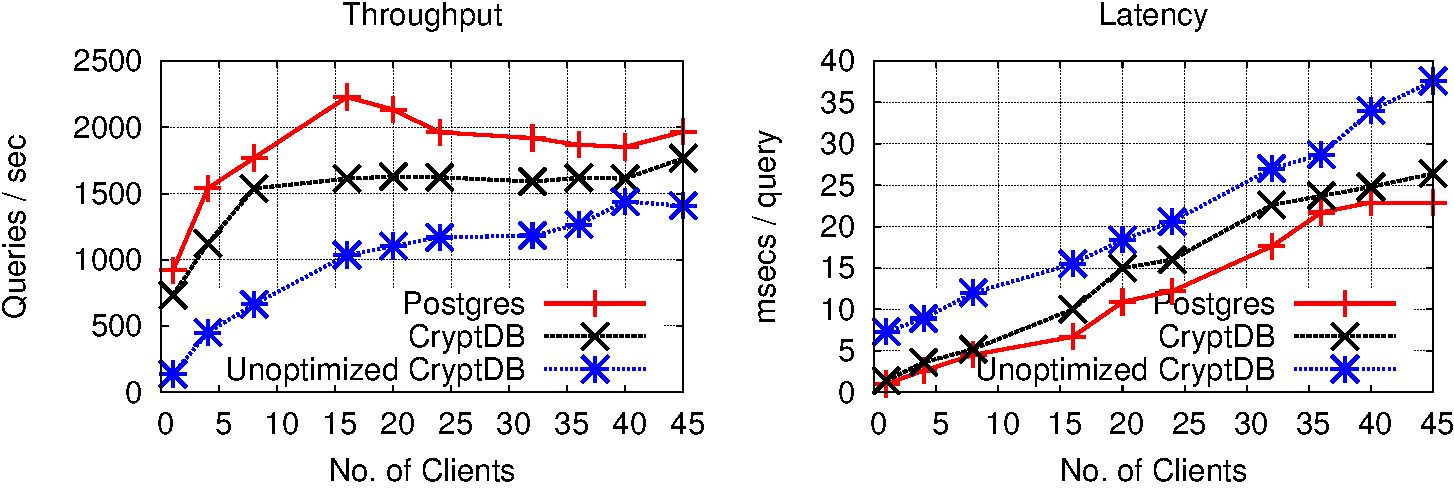
\includegraphics[width=3.5in]{fig/queries.pdf}
\caption{Throughput and latency for TPC-C queries without transactions,
    as a function of the number of concurrent clients.}
\label{fig:querytputlat}
\end{figure}

\begin{figure}[t!] 
\centering
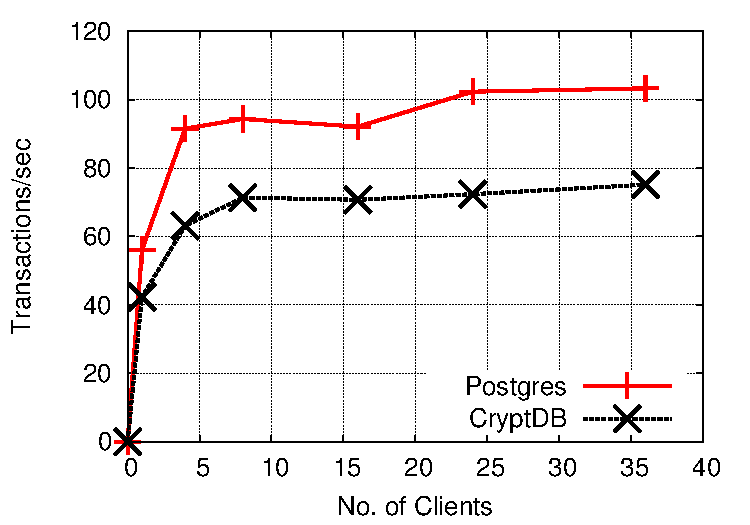
\includegraphics[width=3in]{fig/trantput.pdf} 
\caption{Throughput of TPC-C transactions as a function of
	 the number of concurrent clients.}
\label{fig:trantput}
\end{figure}


Figure~\ref{fig:trantput} shows the throughput achieved for the
TPC-C query mix when transactions are enabled.  In this case,
CryptDB incurs a $27\%$ penalty in terms of throughput compared
to unmodified Postgres, largely due to increased transaction
contention because of longer client-side processing times and
expanded queries.  In case of unoptimized CryptDB, client-side
processing times for each query are increased even further,
leading to significantly more transaction conflicts and an
overall throughput reduction of $70\%$.


\subsection{Query Microbenchmarks}

To understand the sources of overhead incurred by CryptDB, we
examined the throughput of individual queries, since different
applications may result in various query mixes. 
For each query type, we collected corresponding queries from TPC-C,
and measured the latency for those queries running
under CryptDB and under unmodified Postgres.
The results of this experiment are shown in Table~\ref{t:microlat}.
We can see that the client encryption time is generally low, adding
an average of $0.34$ ms to the query.  The unoptimized CryptDB also
has low latency except for queries requiring $\OPE$ and $\HOM$; the
overall client latency of $7.3$~ms may still be acceptable for some
applications.  The fact that server latencies are similar for CryptDB
and unmodified Postgres suggests that the expansion factor due to
encryption has a moderate impact on performance.
In summary, overall CryptDB adds $0.64$~ms of latency to each query,
and unoptimized CryptDB adds $7.6$~ms.

Figure~\ref{fig:microtput} shows the throughput for the same mix of
queries running under CryptDB and unmodified Postgres.  We can see that
for six query types (Select equality, Select join, Select range,
Delete, Insert, and Update set), the throughput overhead is minimal.
These six query types constitute most of the queries both for TPC-C
and likely for many other applications, making CryptDB a good choice.
Homomorphic operations, such as Select sum and Update increment, incur
a significant overhead with CryptDB, due to the server-side cost to
homomorphically multiply large cryptographic numbers instead of adding $32$-bit
integers.  Applications that use sums and increments heavily would incur
significant overhead with CryptDB, but applications with a low percentage
of sums (such as in TPC-C), CryptDB overheads would be much lower.

In terms of storage, the frontends only need to store one master key,
the schema and onion status, as well as ciphertext caches for $\OPE$
and $\HOM$ as an optimization.  For TPC-C queries, the memory footprint
of the frontend process is minimal: $92$~kB of memory, not including
the code and shared libraries like libc, or less than $4$~MB of memory
including code and shared libraries. If the frontend decides to cache ciphertext
for $\OPE$ and $\HOM$, to cache $100000$ values (presumably the most common), it
takes $ < 1$ MB for $\OPE$ and $\approx 12$ MB for $\HOM$.

On the server side, CryptDB increases the size of the database due to
multiple onions and ciphertext expansion.  For TPC-C, the database size
using unmodified Postgres was $135$~MB and with CryptDB, it was $619$~MB,
amounting to $4.5$ times increase. This is mostly because of aggregates
which are large cryptographic numbers, without which it is a three fold increase.
Since disk space is relatively cheap, we do not consider increased
storage cost to be a significant barrier to adoption of CryptDB\@.
CryptDB's runtime overheads are significantly less than the storage
expansion factor because reading a column (or evaluating a predicate
on a column) requires accessing only one of the onions for that column,
instead of every onion for that column.
Moreover, there is virtually no expansion for large data items such as
long strings or binaries.  Therefore, a database storing large text
or binaries (e.g., photos) will have almost no storage overheads.


\begin{table}[t!]
\centering
\begin{tabular}{l|c|c|c|c}

\multirow{2}{*}{Query} & \multicolumn{3}{c|}{CryptDB} & \small{Postgres} \\
\cline{2-5}
& \small{Server} & \small{Client} & \small{Client Unopt.} & \small{Server
} \\
\hline
Select equality    &   0.43    &  0.10   &                 0.10   &  0.41  \\    
Select join   &   0.72    &   0.27    &           0.27       &  0.63   \\          
Select range  &   1.2    &    0.40     &             58.2    &  0.99   \\       
Select sum     &   8.8    &    0.18   &           0.18   &  0.46   \\
Delete       &   1.1    &      0.15   &           0.14       &  1.1   \\                
Insert        &   1.0    &     0.34   &           18.6    &  0.99   \\                                  
Update set     &   1.2    &     0.17   &          0.17   &  1.1   \\                                  
Update increment     &   2.0     &  0.71 &         17.7       &   1.8   \\                         
\hline 
Overall      &       1.4         &  0.34  &         7.3        &  1.1   \\

\end{tabular}
\caption{Latency figures in milliseconds.  The client latency is the encryption
time for CryptDB and unoptimized CryptDB\@.  The overall time reflects the average
latencies for the mixture of TPC-C queries.  ``Update set'' indicates an update
where fields are set to a constant, and ``Update increment'' indicates an update
where fields are incremented.}
\label{t:microlat}
\end{table}


\begin{figure}[t!] 
\centering
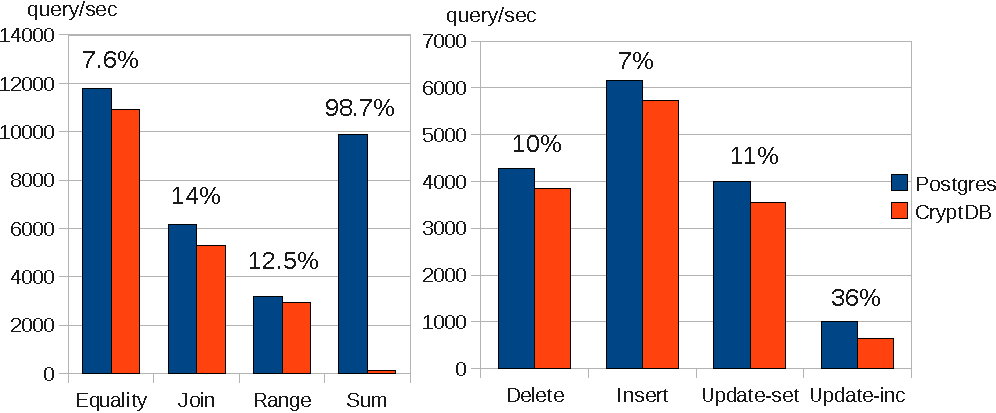
\includegraphics[width=3.4in]{fig/tput.pdf} 
\caption{Throughput comparison for query types from
    Table~\ref{t:microlat} running under CryptDB and
    unmodified Postgres.  For each query type we
    show the percentage throughput reduction under
    CryptDB as compared to unmodified Postgres.}
\label{fig:microtput}
\end{figure}


\subsection{Adjustable Query-based Encryption}


% \begin{figure}[t!] 
% \centering
% 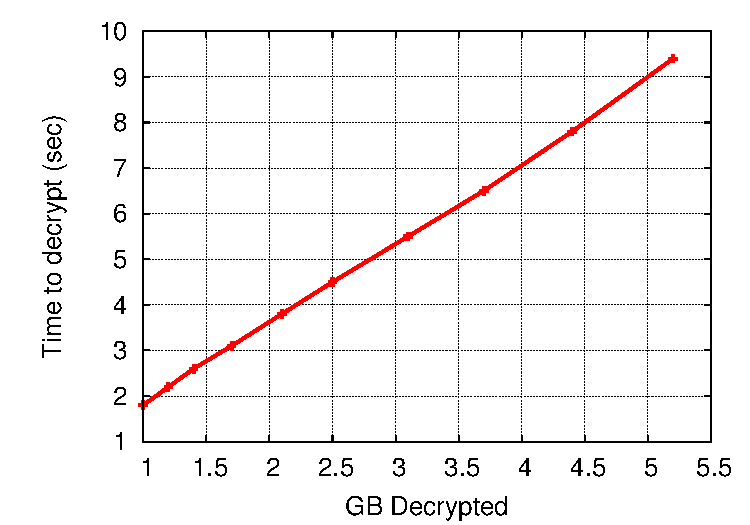
\includegraphics[width=2in]{fig/dec.pdf} 
% \caption{Time to decrypt a column.}
% \label{fig:dec}
% \end{figure}

Adjustable security involves decrypting columns to lower onion levels.
Fortunately, such decryption itself is fast, and only needs to be
performed once per column for the lifetime of the system.  In particular,
in our implementation, removing a layer of $\RND$ encryption requires
decrypting AES, which our server can perform at approximately $500$~MB/sec.
Thus, the cost of removing an onion layer of encryption is
bottlenecked by the speed at which the DBMS server can copy an entire
column of data in a single table; the decryption speed is negligible in
comparison with disk read and write bandwidth.

Table \ref{t:onion} shows the resulting state of the encryption levels of
the various fields in TPC-C's schema after executing the TPC-C queries.
We can see that $71\%$ of the columns remain at
$\RND$ which means that no information leak about them whatsoever. This
shows the importance of dynamically adjusting encryption based on queries rather than
just starting out with encryption that enables all operations. For $\OPE$ only,
$2$ columns have range queries, the other $6$ are decrypted to $\OPE$ due to
\texttt{ORDER BY}. One could avoid such decryption by simply ordering the items
on the frontend.

\begin{table}
\centering
\begin{tabular}{c|c|c|c|c}
$\RND$ & $\DET$ but not $\OPE$ & $\OPE$ & Uses $\HOM$ & Total\\
\hline
 65 &  19 & 8 & 8 & 92 \\
\end{tabular}
\caption{Resulting onion state of the database for TPC-C.}
\label{t:onion}
\end{table}



\subsection{Server Portability}
\label{ss:mysqlport}

To demonstrate the portability of CryptDB, we ported
CryptDB to MySQL\@.  We only had to change and add a total
of $86$ lines of code.  This code was mostly connection code,
allowing the CryptDB frontend to connect to the MySQL server,
a new format for UDF declarations (though the content
was the same), and different handling of information sent to and
received from the server.  However, we did not change any of
the DBMS code in the MySQL server, and did not change any code
for CryptDB's logic in the frontend.  This suggests that CryptDB
can be easily ported to other DBMS servers that support UDFs.



\subsection{Application Portability}

To demonstrate the portability of existing applications to
CryptDB, we ran several applications on CryptDB,
including TPC-C and two different versions of an academic institution's 
graduate admissions web application, one written using hand-written SQL
queries and one
written using the Django ORM system~\cite{bib:django} for Python.  CryptDB
was able to support all SQL queries from these applications without having
to modify the queries or the application in any way. 



% must eval adjustable sec!!




